\documentclass[9pt,twocolumn,twoside]{../../styles/osajnl} 
\usepackage{fancyvrb}
\journal{i524}  

\title{Globus Toolkit} 

\author[1,*]{Saber Sheybani} 

\affil[1]{School of Informatics and Computing, Bloomington, IN 47408, U.S.A.} 

\affil[*]{Corresponding authors: sheybani@indiana.edu} 

\dates{paper-001, \today} 

\ociscodes{Globus Toolkit, grid computing, WSRF, OGSA, cluster resource management} 

\doi{\url{https://github.com/ssheybani/sp17-i524/tree/master/paper1/S17-ER-1001/report.pdf}} 


\begin{abstract} 
The Globus Toolkit is an open source software stack, developed to serve as the middleware for grid computing. It is organized as a collection of loosely coupled components consisting of services, programming libraries and development tools designed for building grid-based applications. GT components fall into five broad domain areas: Security, Data Management, Execution Management, Information Services, and Common Runtime.\newline
\end{abstract} 

\setboolean{displaycopyright}{true} 

\begin{document} 

\maketitle 

\section{Introduction} 

Initially, work on Globus was motivated by the demands of "virtual organizations" in science. These organizations need access to resources and services which are not easily replicable locally. Examples of these needs include access and management of equipment and large amounts of data, located in various remote databases on a regular basis. Although each application may have different specific requirements, the demand for a few basic functions is shared between most applications. "They often need to discover available resources, configure a computing resource to run an application, move data reliably from one site to another, monitor system components, control who can do what, and manage user credentials". These functions can be well addressed in a grid computing framework \cite{foster2006globus}.

According to \cite{sotomayor2006globus}, ``\emph{a \textbf{grid} is a system that coordinates resources that are not subject to centralized control, using standard, open, general-purpose protocols and interfaces to deliver nontrivial qualities of service}''. The major difference between grids and other distributed systems is that grids have significantly larger extent of heterogeneity of resources. They also enable resource sharing among virtual organizations, whereas other distributed computing technologies only support a single organization \cite{magoules2009introduction}. The grid architecture consists of a number of layers that altogether serve the functions and purposes of the systems (See figure \ref{fig:grid-arch}). EGEE: Enabling Grids for E-Science in Europe \cite{egee-web}, NEESit: Network for Earthquake Engineering Simulation \cite{neesit-web}, TeraGrid \cite{teragrid-wiki} are examples of grid systems.
\begin{figure}[htbp]
\centering
\fbox{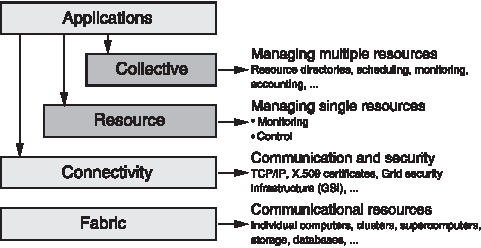
\includegraphics[width=\linewidth]{images/fig1}}
\caption{Grid Architecture \cite{sotomayor2006globus}}
\label{fig:grid-arch}
\end{figure}

A grid system often comprises various services such as Job Management Service and Resource Discovery and Management Service, which constantly need to interact with each other. However, each of these services may have been implemented by different vendors, which is not necessarily compatible with other services. The \textbf{Open Grid Services Architecture (OGSA)} aims to standardize practically all the services that can commonly be found in a
grid system (job management services, resource management services, security services, etc.) by specifying a set of standard interfaces for these services.
In order to realize that goal, OGSA needs to choose some sort of distributed middleware on which to base the architecture. In other words, if OGSA (for example) defines that the JobSubmissionInterface has a submitJob operation, there has to be a common and standard way to invoke that operation. \textbf{Web Services} were chosen as the underlying technology. Web services are platform-independent and language-independent since they are message-oriented and rely on language-neutral XML dialects to send messages, to specify interfaces, etc. Hence, web services are well-suited for building loosely coupled systems such as grid systems.

However, although Web services can, in theory, be either stateless or stateful, they are usually stateless. This means that the Web service can’t "remember" information, or keep state, from one invocation to another. On the other hand, OGSA requires Stateful Services. 
The \textbf{Web Services Resource Framework (WSRF)} specifies how we can make our Web Services stateful, along with adding other features. In other words, while OGSA is the architecture, WSRF is the infrastructure on which that architecture is built on.

With this background, we can define Globus Toolkit as an open source toolkit that provides an implementation of OGSA, WSRF and a number of other standards for grid computing. Figure \ref{fig:relation} displays the relationship between OGSA, Web service, WSRF, Globus Toolkit.
\begin{figure}[htbp]
\centering
\fbox{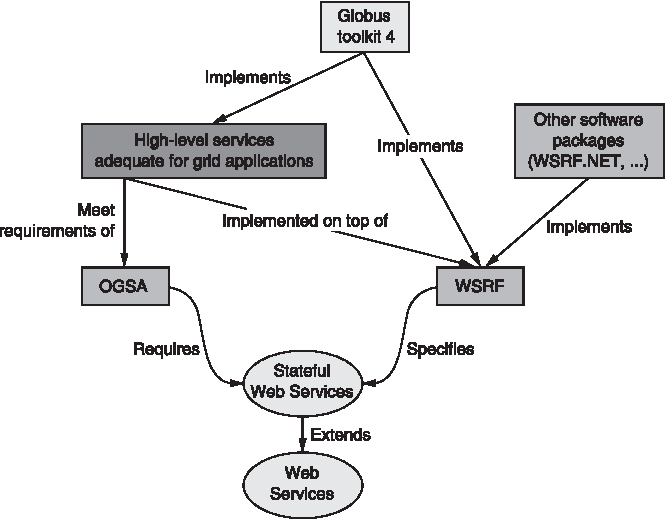
\includegraphics[width=\linewidth]{images/fig2}}
\caption{Relationship between OGSA, GT4, WSRF, and Web Services \cite{sotomayor2006globus}}
\label{fig:relation}
\end{figure}

\section{Components} 

The libraries and services in Globus Toolkit can be classified into five broad domain areas, namely security, data management, execution management, information services, and common runtime. Components in each of these areas will be discussed further in this section \cite{sotomayor2006globus}.
\begin{description}

\item[Security]: Grid Security Infrastructure (GSI) is a collection of components in GT4 that facilitate secure communication in the system. These components include authentication and authorization (for controlling access to services and resources), delegation, community authorization, and credential management.

\item[Data Management]: These components provide for the discovery, transfer, and access to large data. They include GridFTP (an implementation of a protocol optimized for transferring large amounts of data between hosts), Reliable File Transfer (adds several features to GridFTP), Replica Location Service(keeping track of different replicas of a dataset in a virtual organization), Data Replication (uses RLS, RFT to guarantee that local copies of replicas are available to the hosts), and OGSA Data Access and Integration (a framework to access and integrate datasets on a Grid).

\item[Execution Management]: These components handle the deployment, scheduling, and monitoring of executable programs, referred to as jobs. They include Grid Resource Allocation and Management (the heart of GT Execution Management, providing services to deploy and monitor jobs), Community Scheduler Framework (provides a single interface to different resource schedulers), Workspace Management (allows users to dynamically create and manage workspaces on remote hosts), and Grid Telecontrol Protocol (provides a WSRF-enabled service interface for control of remote instruments).  

\item[Information Services]: Commonly referred to as the Monitoring and Discovery System (MDS), these services deal with monitoring and discovery of resources in a virtual organization. They include Index Service(for aggregation of resources of interest to a VO), Trigger Service (same as Index Service, but is configured to perform certain actions based on the data collected from resources), and WebMDS (provides a web browser-based view of data collected by GT4 aggregator services).

\item[Common Runtime]: These components provide a set of fundamental libraries and tools for hosting existing services as well as developing new services, in languages of C, Java, and Python (C Runtime, Java Runtime, and Python Runtime).

\end{description}

\section{Applications}
Globus Toolkit has been used in many scientific and industrial applications. Examples of large-scale e-science projects relying on the Globus Toolkit include the Network for Earthquake Engineering and Simulation (NEES), FusionGrid, the Earth System Grid (ESG), the NSF Middleware Initiative and its GRIDS Center, and the National Virtual Observatory. In the design of the Large Hadron Collider at CERN, Globus-based technologies have been developed through the European Data Grid, and the U.S. efforts like the Grid Physics Network (GriPhyN) and Particle Physics Data Grid \cite{www-about-globus}.

Globus Toolkit is helping to bridge the gap for commercial applications of Grid computing. Thus, companies like Avaki, DataSynapse, Entropia, Fujitsu, Hewlett-Packard, IBM, NEC, Oracle, Platform, Sun, and United Devices have pursued Grid strategies based on the Globus Toolkit. 
A company named Univa Corporation is devoted to providing commercial support for Globus software. In addition, the Globus Consortium was formed by a group of companies with an interest in supporting Globus Toolkit enhancements for enterprise use \cite{www-about-globus}.

\section{Ecosystem and support}
Globus Toolkit is a part of the larger "Globus ecosystem", which provides a wide range of application-level functions in many domains. Other than the GT, the ecosystem includes a number of other tools, a resource provider and a community of users and developers \cite{foster2006globus}.

Support for Globus ecosystem includes documentation, software updates, mailing lists, and training. The documentation includes manuals, specific for general use, system administrators, developers, and end user. In addition, many tutorials, papers, and presentations are accessible on the website \cite{www-globus-tutorial}. Workshops and conferences for in-person learning are also available. For Java developers, \cite{sotomayor2006globus} is a specifically useful resource for learning how to implement a grid using GT from scratch.

\section{Related Software}
There is a number of software available for use with certain versions of GT, in order to extend the abilities of each of its components. Here are a few examples of each: GridShib and PERMIs for security, Weka4WS for data management, HandleSystem-GT Project for information services, Condor-G, GridWay and Sun Grid Engine for execution management, Grid Packaging Tools (GPT) for packaging, pyGridware, Java CoG Kit and WSRF.NET for programming, and Common TeraGrid Software Stack (CTSS) and LHC Computing Grid (LCG) for software distributions. The full list of software is available in [www-related-tools].


\section{Comparison}
Currently, there are multiple versions of grid middleware stacks. In \cite{schwiegelshohn2010perspectives}, it is argued that none of the available stacks is generally accepted
by all user communities. However, started in 1996, the Globus project is the first grid middleware created \cite{www-uchigago} and has managed to keep a large community of users. Figure \ref{fig:comp-table} shows a comparison of GT and three other grid middleware technologies, namely UNICORE, Legion, and Gridbus. Efforts have been made to combine GT and UNICORE, in order to get the best of both of them \cite{rambadt2002unicore}.
\begin{figure}[htbp]
\centering
\fbox{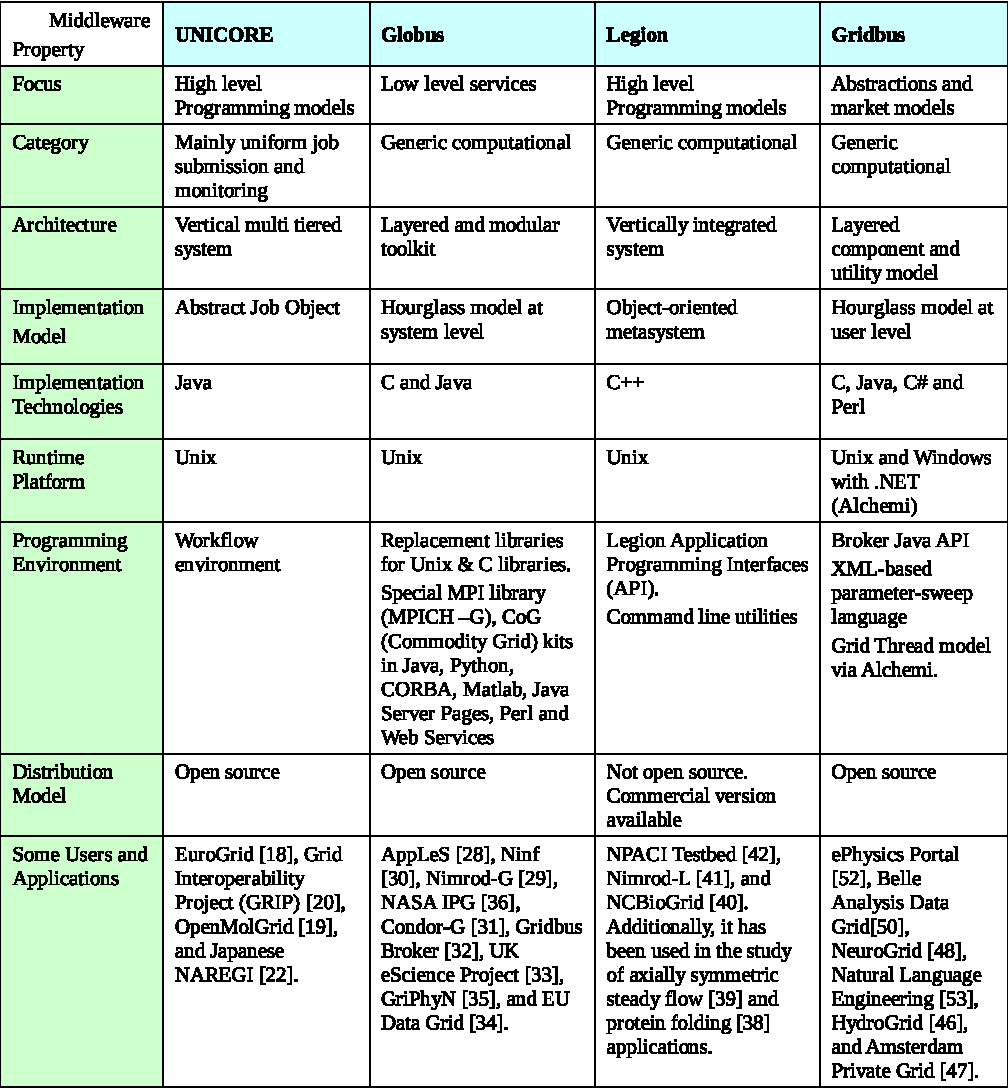
\includegraphics[width=\linewidth]{images/fig3}}
\caption{Comparison of Grid Middleware Systems \cite{asadzadeh2005global}}
\label{fig:comp-table}
\end{figure}

\section{Conclusion}
Globus toolkit is a collection of tools for building grid computing networks, which is a suitable solution for distributed computing. 
It provides APIs for languages of C, Python, and Java. It is the most widely used grid middleware, in comparison to its competitors 
and has been used in many notable scientific and industrial projects. Extensive documentations and tutorials are available for beginners to start using Globus Toolkit.


\section{Acknowledgement}
The author would like to thank Professor Gregor von Laszewski and the
teaching assistants for all the support and guidance. This paper is written during spring of 2017
semester course {I524: Big Data and Open Source Software Projects} at
Indiana University Bloomington.

% Bibliography 
\bibliography{references}

\end{document}
